\documentclass{article}
\setlength{\parskip}{5pt} % esp. entre parrafos
\setlength{\parindent}{0pt} % esp. al inicio de un parrafo
\usepackage{amsmath} % mates
\usepackage[sort&compress,numbers]{natbib} % referencias
\usepackage{url} % que las URLs se vean lindos
\usepackage[top=25mm,left=20mm,right=20mm,bottom=25mm]{geometry} % margenes
\usepackage{hyperref} % ligas de URLs
\usepackage{graphicx} % poner figuras
\usepackage[spanish]{babel} % otros idiomas
\usepackage{textcomp}
\usepackage{pgfplots} % crear graficas
\pgfplotsset{width=9cm,compat=1.7}

\title{"P0"} %titulo
\author{NESTOR RODRIGUEZ} % author
\date{January 2022}

\begin{document} % inicia contenido

\maketitle % cabecera

\begin{abstract} % resumen
  Practica sencilla y unica de un demo del uso de LATEX en
  Overleaf.
\end{abstract}

\section{Introducci\'{o}n}\label{intro} % seccion y etiqueta



Esta practica es un ejemplo de como realizar los reportes de nuestras tareas. Vamos a incluir una ecuacion \eqref{equ}:

\begin{equation}
  f(x) = 10 \tanh(x) - \int_0^\infty \frac{5}{10 + x} \text{d}x.
  \label{equ}
\end{equation}

Tambien podemos citar fuentes. Al final se incluye la figura de una orquidea en la figura \ref{flor}. Vamos a aprender ademas a citar fuentes {ejemplo}.
Se incluye unas tablas \ref{datos} con algunos datos y en la figura \citep{imagen} \ref{flor} hay una orquidea.

\begin{figure} % figura
    \centering
    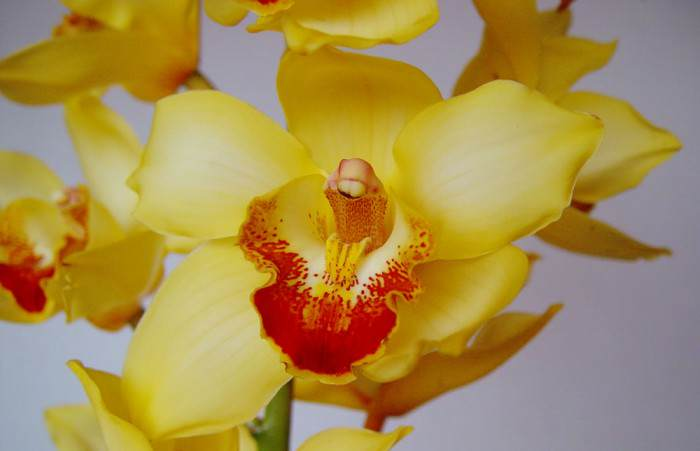
\includegraphics [width=90mm]{orchid.jpg} % archivo
    \caption{orchid recuperada de \url{https://www.floresyplantas.net/orquidea-cymbidium/} con licencia CC.}
    \label{flor}
\end{figure}

\newpage

\section{Creacion de tablas y cuadros}

En esta secci\'{o}n se aprende a crear tablas y cuadros.

\begin{table}[h!] % cuadro
    \caption{Cuadro comparativo de reacciones químicas} % explicacion
    \label{datos} % etiqueta
    \centering % centrar
    \begin{tabular}{l|cr} % izq sep centrada der
         NP Permanganato de sodio & $\beta$ & 8.2230 \\
         NP Oxido de gadolinio  & $\alpha$ & 236.9102 \\
         NP Titanato de Bario & $\Gamma$ & 15.5690 \\
         NP Silicato de Calcio & $\epsilon$ & 89.1691 \\
         NP Nanocelulosa & $\Delta$ & 321.7810 \\
         NP Hidrato Cloruro de Magnesio & $\Omega$ & 101.3010 
    \end{tabular}
\end{table}

\begin{table}[h!]

    \caption{Tablas.}
    \label{otros_datos}
    \centering
    \begin{tabular}{c|c|c|c|c|c||c|c|}
      Dato 1 & Dato 2 & $\Omega$ & Dato 3 \\
      NP 1 & NP 2 & $\pi$ & NP 3 \\
      Resultado 1  &   Resultado 2   &   $\alpha$ &  Resultado 3 
    
    \end{tabular}
\end{table}

\subsection{Midiendo en R}

Se demostrará las secuencias donde se muestra la tabla de las mediciones en los siguientes parámetros logrando el tamaño en nanometros en medición R.

\begin{table}[h!]
    \centering
    \caption{Medidas de tiempo y tamaño en R}
    \begin{tabular}{|c|c|c|c||c|c|c|c||c|c|c|c|}
    \hline
       Matrices  & Datos & Tiempo (s) & Tamaño (nm) & Observaciones  \\
       \hline\hline
        1 & 9560 & $<$ 0.01 & 8024703 & El dato resultado es menor a 1.09 \\
        \hline
        2 & 120 & $<$ 1.20 & 3780164 & El dato resultado es mayor a 1.20 \\
        \hline
        3 & 2360 &  1.03 & 9113822 & El dato resultado es menor a 1.03 \\
        \hline
        4 & 2048 & $<$ 2.40 & 1265499 & El dato resultado es mayor a 2.40\\
        \hline
        5 & 4096 & 3.01 & 4708691 & El dato resultado es menor a 1\\
        \hline
        6 & 9600 & 1.02 & 9410875 & El dato resultado es mayor a 1 \\
        \hline
        7 & 9900 & 4.20 & 9782103 & El dato resultado es igual a 2.0\\
        \hline
        8 & 9703 & 4.90 & 9587023 & El dato resultado es mayor a 4.0 \\
        \hline
        9 & 9380 & 5.10 & 9032458 & El dato resultado es mayor a 5.0 \\
        \hline
        10 & 9060 & 5.94 & 7598013 & El dato resultado es mayor a 1.0\\
        \hline
        11 & 9799 & 5.85 & 8712039 & El dato resultado es mayor a 1.0\\
        \hline
    \end{tabular}
    \label{medir_R}
\end{table}

\subsection{Midiendo en Python}

Se observa la siguiente tabla en la distribucion de la medicion en los vectores en Python.

\begin{table}[h!]
    \centering
    \caption{Mediciones en tiempo, tamaño y real en Python}
    \begin{tabular}{|c|c|c|c||c|c|c|c||c|c|c|c|}
    \hline
       Datos & Tiempo (s) & Tamaño (nm) & Real  \\
       \hline\hline
        1 & 9560 & $<$ 0.01 & 8024703 \\
        \hline
        2 & 120 & $<$ 1.20 & 3780164 \\
        \hline
        3 & 2360 &  1.03 & 9113822 \\
        \hline
        4 & 2048 & $<$ 2.40 & 1265499 \\
        \hline
        5 & 4096 & 3.01 & 4708691 \\
        \hline
        6 & 9600 & 1.02 & 9410875 \\
        \hline
        7 & 9900 & 4.20 & 9782103 \\
        \hline
        8 & 9703 & 4.90 & 9587023 \\
        \hline
        9 & 9380 & 5.10 & 9032458 \\
        \hline
        10 & 9060 & 5.94 & 7598013 \\
        \hline
        11 & 9799 & 5.85 & 8712039 \\
        \hline
    \end{tabular}
    \label{medir_R}
\end{table}

\section{Grafica}



En esta parte se aprenderá a como utilizar y hacer una grafica en LATEX

\begin{center}
\begin{tikzpicture}
\begin{axis}[
title={Absorbancia  de la corrosion de H2SO4 con la Temperatura},
xlabel={Temperatura \textcelsius},
ylabel={Absorbancia anticorrosiva ml de clorato},
xmin=0, xmax=300,
ymin=0, ymax=200,
={0,20,40,60,80,100,110,120,130,140,150},
={0,20,30,40,50,60,70,80,90,100,110,120},
={10,20,30,40,50,60,70}
legend pos=north west,
ymajorgrids=false,
grid style=dashed,
]
\addplot[
color=blue,
mark=square,
]
coordinates{
(0,0)(10,10)(20,30)(40,39.8)(60,64.6)(80,72.8)(130,93.8)(170,140)(250,140)
};
\legend{H2SO4}

\end{axis}
\end{tikzpicture}
\end{center}

\section{Conclusion}

En general todo el desarrollo de este documento me sirvió de práctica que me permitió explorar más a fondo las funciones que tiene el programa, además de familiarizarme con su interfaz, comandos y también obtuve más práctica con este programa. Aún así mismo considero que aún tengo mucho que aprender en cuanto a programación de códigos, dado que tuve muchas dificultades, batalle pero se logro el objetivo para aprender en esta parte para trabajar en Overleaf.

\section{Referencias}
\cite
{Latex allergy}
  title={},
  author={Slater, Jay E},
  journal={Journal of Allergy and Clinical Immunology},
  volume={94},
  number={2},
  pages={139--149},
  year={1994},
  publisher={St. Louis, MO: CV Mosby Co., c1971-}



\bibliography{bib}
\bibliographystyle{plain}

\end{document}
